\documentclass[a4paper,twoside]{article}
\usepackage{autiwa}
\title{Trucs astuces de photographie numérique}
\author{Autiwa}
\makeindex
\begin{document}
\begin{titlepage}
\begin{center}
~
\vfill
% Upper part of the page
\begin{figure}[t]
\centering
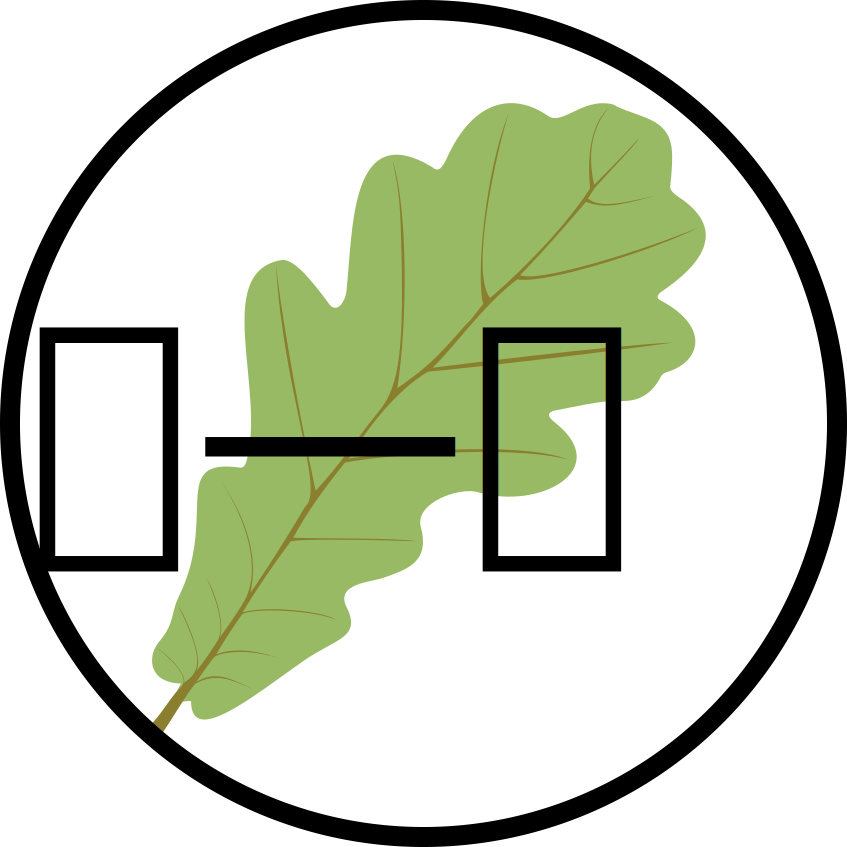
\includegraphics[width=0.15\textwidth]{logo-autiwa.pdf}%chemin absolu de l'image pour que l'on puisse appeler ce fichier depuis plusieurs dossiers différents.
\end{figure}

% Title
\HRule \\[0.4cm]
{ \huge \bfseries \makeatletter\@title\makeatother}\\[0.4cm]

\HRule \\[0.75cm]
{\large \today}\\[0.75cm]
\makeatletter
\@author
\makeatother
\vfill
\vfill
~
% Bottom of the page


\end{center}
\end{titlepage}

\tableofcontents
\newpage
\section{Introduction}
Ce document a pour but de compiler des trucs et astuces pour la photo numérique, et d'expliquer les choses basique qu'il faut maîtriser. Il n'a pas pour but d'être exhaustif, mais plutôt de servir d'aide mémoire. 

Il expliquera le fonctionnement de l'appareil en se basant sur le \textbf{Canon EOS 7D}. Beaucoup de choses restent cependant valables quel que soit l'appareil.

\bigskip

Une partie minuscule tout de suite pour parler des accessoires indispensables ou quasiment indispensable :
\begin{itemize}\index{matérial indispensable}
\item Une batterie de rechange. C'est bête à dire, mais ça peut sauver une session photo
\item un flash externe. En plus, avec le 7D, on peut le contrôler à distance
\item une télécommande pour pouvoir faire des poses longues
\item une alimentation externe, afin de pouvoir faire des photos sur trépieds, chez soi, sans être préoccupé par le manque de batterie
\item ne pas négliger la qualité de la carte mémoire, et en particulier sa rapidité. C'est très important pour le mode rafale et le mode vidéo par exemple.
\item un disque dur nomade multimédia sur lequel on peut directement brancher les cartes compact flash pour les vider de leur contenu.
\end{itemize}

\begin{remarque}
Une remarque générale sur le matériel. Il faut penser à chercher sur internet des tests et comparaisons, c'est parfois crucial pour trouver le meilleur rapport qualité prix ou pour éliminer de suite certaines marques dont les produits ne sont pas fiables, ou inférieurs.
\end{remarque}

\begin{attention}
Le \textbf{Quick Control Dial}, la molette avec le bouton \og SET\fg au milieu a une position \textbf{lock}. Cette dernière empêchera la modifiction de l'ouverture dans les modes \textbf{M} et \textbf{B}
\end{attention}

\section{Les bases}
\subsection{La profondeur de champ}
La profondeur de champ c’est une zone de netteté qui s’étend en deçà et au delà du plan de netteté. \emph{Elle se repartit 1/3 devant et 2/3 derrière. Les objets situés en dehors de la profondeur de champ seront flous sur l’image.} C'est en fait simplement la zone à l'intérieur de laquelle le cercle de confusion des rayons provenant d'un même point de l'image est plus petite qu'un pixel. Quand ce n'est plus le cas, l'image est floue.

\begin{remarque}
Le cercle de confusion est dû au fait qu'un élément d'optique ne donnera pas une focalisation ponctuelle d'une image ponctuelle, même après focalisation. Ce petit cercle contenant tous les rayons lumineux d'un même point objet permet de déterminre, en comparant à la taille de pixel, si ce point sera net ou pas.
\end{remarque}


\begin{figure}[htb]
\centering
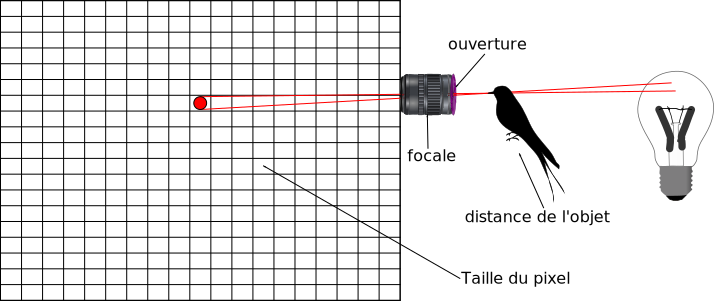
\includegraphics[width=0.5\linewidth]{figure/confusion_circle.pdf}
\caption{Schéma représentant le trajet lumineux de tous les rayons éclairant un même point de l'image source. Ces rayons se retrouvent dans ce qu'on appelle un cercle de confusion une fois la mise au point faite. Si ce cercle de confusion se trouve être plus petit qu'un pixel de l'appareil photo, alors ce point apparaîtra net, sinon il apparaîtra flou. Sur le schéma sont représentés les différents paramètres qui vont modifier la profondeur de champ, c'est à dire la zone de l'image dans laquelle le cercle de confusion sera plus petit qu'un pixel. Ces paramètres sont la distance de l'objet, la focale de l'objectif, la taille du pixel et l'ouverture.}
\end{figure}

Cette zone est fonction de 4 paramètres essentiellement :
\begin{itemize}
\item l'\textbf{ouverture} du diaphragme : Plus l'ouverture est grande et plus le cône de lumière entrant dans l'objectif pour un point donné aura un angle d'ouverture grand. Ainsi, le cercle de confusion sera plus grand
\item la \textbf{longueur focale} de l'objectif : Plus la focale est grande et plus la profondeur de champ est faible, (pour tous les autres paramètres fixés)
\item la \textbf{distance de mise au point} : Plus la distance de mise au point est grande, et plus la profondeur de champ est grande
\item le format du capteur : Plus les pixels sont grands, et plus la profondeur de champ est grande.
\end{itemize}

\begin{attention}
Je ne pense pas avoir raison en disant que la référence pour le capteur est la taille du pixel, car où que je regarde sur internet, la valeur a l'air d'être la même pour un type de capteur (full frame par exemple) et ce quel que soit le nombre de pixel total. Je ne comprends donc pas cette partie là, mais vu que c'est une constante, ce n'est pas vraiment important. Pour le 7D ce nombre vaut $0.019\unit{mm}$.
\end{attention}

\begin{important}
Ce qu'il faut retenir : 
\begin{enumerate}
\item La zone de netteté se repartit 1/3 devant et 2/3 derrière à grande distance, sinon c'est plutôt 50--50;
\item Si le diaphragme augmente (c’est-à-dire passer de f/2 à f/16) la profondeur de champ augmente ;
\item Si la focale diminue (c’est-à-dire passer de 50mm à 24mm) la profondeur de champ augmente ;
\item Si la distance de mise au point augmente (passer de 3m à l’infini) la profondeur de champ augmente.
\end{enumerate}
\end{important}

Voici pour 4 focales \reffig{fig:pdc} l'évolution de la profondeur de champ en fonction de la distance du sujet et de l'ouverture de l'objectif. En gros, pour lire ces graphiques, il suffit de déterminer quelle profondeur de champ on veut, par exemple 10cm, regarder à quelle courbe ça correspond, et ensuite, on prend une focale et on lit la distance du sujet correspondante ou inversement.

\begin{figure}[htb]
\centering
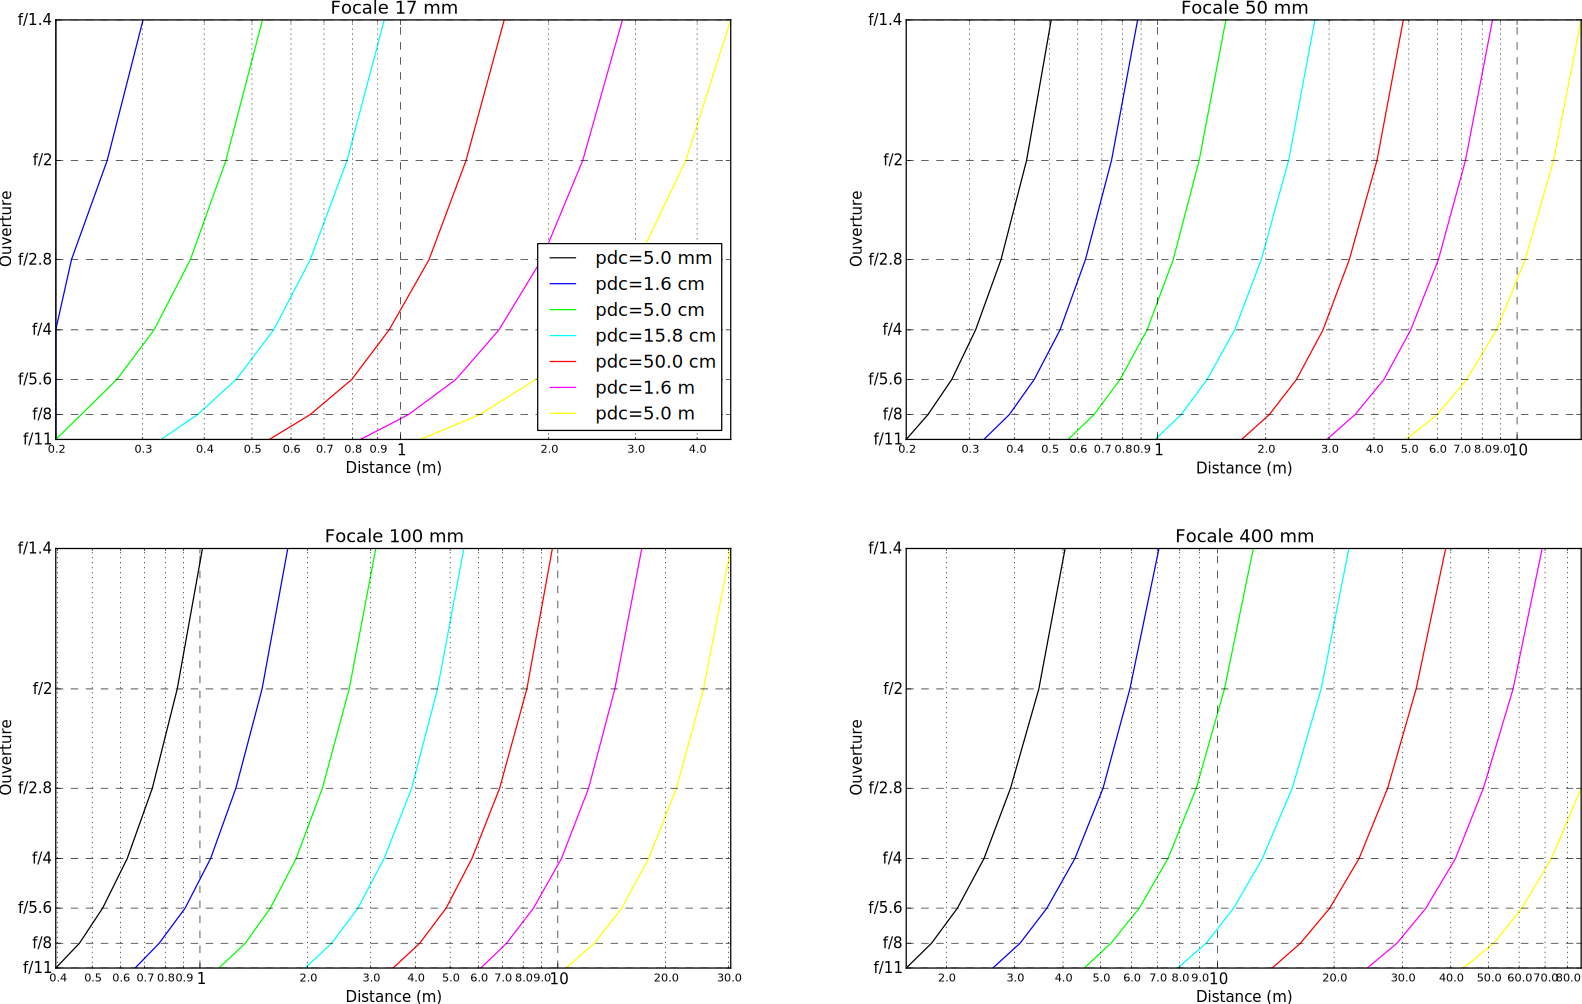
\includegraphics[width=\linewidth]{figure/pdc.pdf}
\caption{Courbes, pour des focales de 17, 50, 100 et 400mm permettant, pour une profondeur de champ donnée, de trouver la correspondance entre l'ouverture et la distance au sujet permettant d'avoir cette valeur de profondeur de champ. Il faut garder à l'esprit que la profondeur de champ est au mieux symétrique autour du sujet, sinon plutôt 1/3 devant et 2/3 derrière.}\label{fig:pdc}
\end{figure}

%TODO faire un tableau récapitulatif des profondeurs de champ en fonction de la distance du sujet, de l'ouverture, de la focale. Faire des iso profondeur de champ en variant deux paramètres, et en faisant plusieurs graphiques pour faire varier le dernier paramètre.

\subsubsection{Hyperfocale}
L'hyperfocale est la distance minimale de mise au point qui donne une zone de netteté qui s'étend jusqu'à l'infini.

\begin{figure}[htb]
\centering
\includegraphics[width=0.5\linewidth]{figure/hyperfocal.pdf}
\caption{Sur ce graphique est représenté l'hyperfocale (la distance minimale de mise au point qui permet d'avoir une zone de netteté qui s'étend à l'infini) pour différentes valeurs d'ouverture et de focale.}
\end{figure}
%TODO donner un graphique de la valeur de l'hyperfocale pour différentes focales et ouvertures

\subsection{L'exposition}
L'exposition d'une photo, ou dit autrement la quantité de lumière nécessaire pour avoir une image, est déterminée par deux variables : 
\begin{itemize}
\item Le temps d'exposition
\item l'ouverture, exprimée en fraction de la focale (f/5.6 par exemple).
\end{itemize}

À ces paramètres s'ajoute la valeur ISO, c'est à dire la sensibilité du capteur à la lumière. ISO 200 est deux fois plus sensible qu'ISO 100, et il faudra donc deux fois moins de lumière pour que la photo soit correctement exposée, mais en contrepartie, l'image aura un bruit plus important. 

À une valeur d'exposition donnée correspond plusieurs couples vitesse--ouverture comme l'illustres \reffig{fig:exposition-equivalente} et \reftab{tab:exposition-equivalente}

\begin{table}[htb]
\centering
\begin{tabular}{llll}
Vitesse & Ouverture & Vitesse & Ouverture\\\hline
1/30 s & f/22 & 1/1000 s & f/4\\
1/60 s & f/16 & 1/2000 s & f/2.8\\
1/125 s & f/11 & 1/4000 s & f/2\\
1/250 s & f/8 & 1/8000 s & f/1.4\\
1/500 s & f/5.6 
\end{tabular}
\caption{Exemple de couple vitesse d'obturation/ouverture qui donnent la même exposition (pour une sensibilité ISO identique)}\label{tab:exposition-equivalente}
\end{table}

\begin{figure}[htb]
\centering
\includegraphics[width=0.65\linewidth]{figure/exposition.pdf}
\caption{Illustration des équivalences de couples temps de pose/ouverture.}\label{fig:exposition-equivalente}
\end{figure}

\begin{remarque}
Il est important de remarquer que les ouvertures ne sont pas espacées au hasard. Elles sont espacées de sorte que la surface soit doublée ou divisée par deux pour deux valeurs adjacentes. 

De même, les vitesses d'obturations sont incrémentées par un facteur 2 à chaque fois. Ainsi, en prenant l'ouverture immédiatement plus grande, et la vitesse adjacente supérieure, l'exposition reste la même. On double l'ouverture, mais on divise la vitesse par deux, l'exposition reste donc la même.
\end{remarque}

\begin{figure}[htb]
\centering
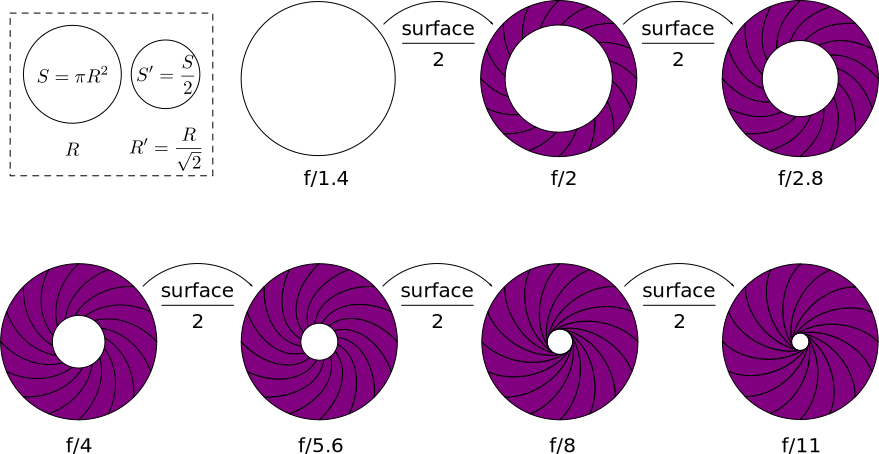
\includegraphics[width=0.65\linewidth]{figure/aperture.pdf}
\caption{Représentation des ouvertures, pour une focale donnée. Un stop d'ouverture fait entrer deux fois plus ou deux fois moins de lumière dans l'appareil.}\label{fig:ouverture}
\end{figure}

\subsubsection{Comment est calculée l'exposition}
La quantité de lumière nécessaire pour qu'un sujet soit correctement exposé dépend de différents facteurs :
\begin{itemize}
\item L'intensité de la lumière ambiante
\item Le pouvoir de réflexion du sujet.
\end{itemize}

En effet, un sujet blanc renvoi beaucoup plus efficacement la lumière qu'on objet noir, ceci doit être pris en compte lors du calcul de l'exposition. Comme l'appareil photo ne peut pas savoir \emph{a priori} la couleur du sujet, les appareils mesurent l'exposition en supposant que c'est un sujet ayant 12--18\% de gris. C'est utile si le sujet comprend des parties blanches, noire et grises par exemple. 

Dans d'autres cas précis, afin d'avoir un sujet correctement exposé, on peut compenser l'exposition via la valeur \textbf{EV} (Exposure Value). Si cette valeur est à 0, on ne compense pas l'exposition, si on la met à une valeur positive, on surexpose la photo, et si on met une valeur négative, on sous-expose. 

Il suffit de passer à la valeur immédiatement supérieure d'exposition ou de vitesse pour augmenter l'EV d'un \textbf{stop}. Vous entendrez souvent ce mot en photographie, ça signifie qu'un facteur 2 a été appliqué soit à l'ouverture, soit à la vitesse d'obturation.

\subsubsection{Contrôler l'exposition avec l'histogramme}
L'histogramme répertorie le nombre de pixel pour chaque luminosité (ou alors par couleur), de la plus sombre à gauche à la plus lumineuse à droite. 

Si la partie de gauche est vide de pixel, la photo est surexposée. Si la partie de droite est vide, la photo est sous exposée. 

L'idée est d'avoir la plage entière de valeur remplie, et les bords avec peu de pixels.

\subsection{Mesure de l'exposition}
\subsubsection{Évaluative}
L'image est découpée en 63 zones, représentées par des rectangles jaunes sur \reffig{fig:metering-evaluative}. La mesure de l'exposition est faite sur les zones, avec un poids plus important pour les zones où la netteté est faite. 

\begin{figure}[htb]
\centering
\subfloat[Mesure évaluative de l'exposition à partir des 63 zones représentées par un rectangle jaune. Les zones où la mise au point est faite auront un poids plus important dans l'évaluation globale.]{\label{fig:metering-evaluative}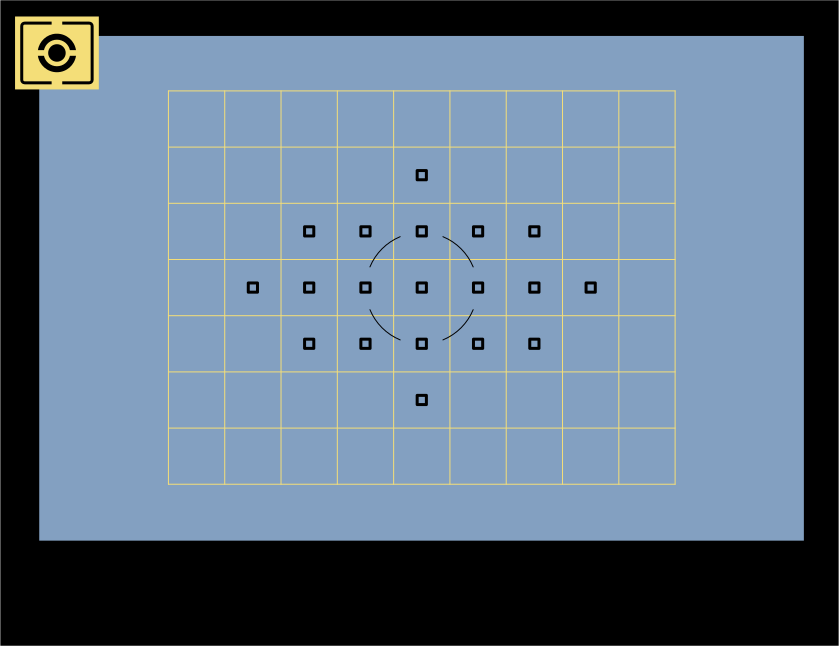
\includegraphics[width=0.45\linewidth]{figure/metering_evaluative.pdf}}\hfill
\subfloat[L'évaluation partielle utilise un spot central qui représente environ 9\% de l'image.]{\label{fig:metering-partial}\includegraphics[width=0.45\linewidth]{figure/metering_partial.pdf}}

\subfloat[L'évaluation par spot base l'exposition sur une zone centrale représentant environ 3\%]{\label{fig:metering-spot}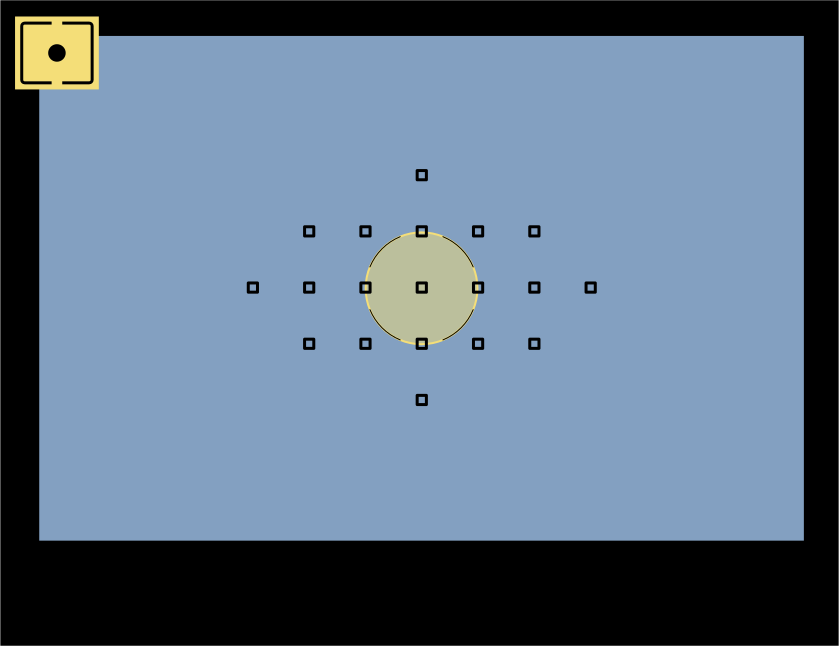
\includegraphics[width=0.45\linewidth]{figure/metering_spot.pdf}}\hfill
\subfloat[Le mode d'évaluation \og central weighted\fg calcule l'exposition à partir de l'image complète, mais donne une importance plus grande à la zone centrale.]{\label{fig:metering-central-weighted}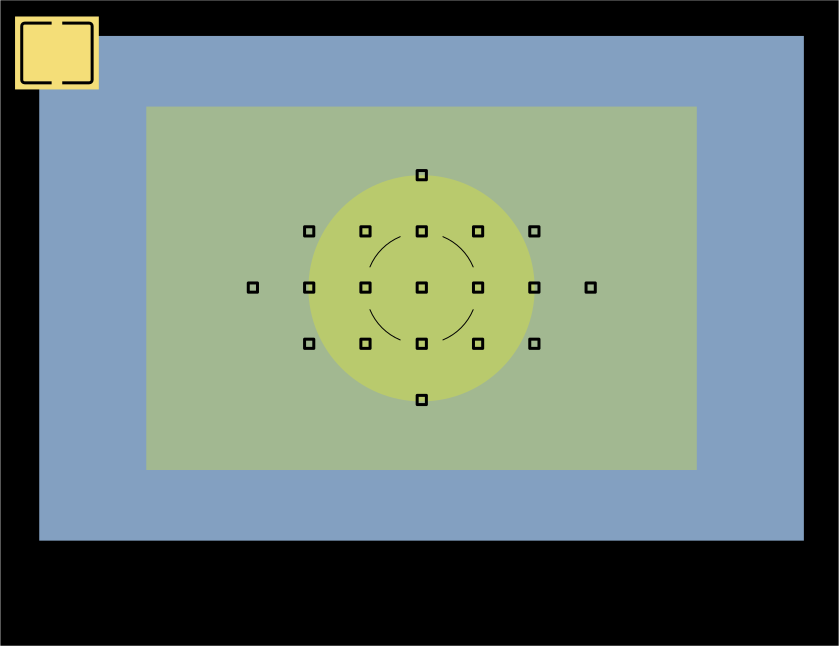
\includegraphics[width=0.45\linewidth]{figure/metering_central_weighted.pdf}}
\caption{Voici les différentes méthodes de mesure de l'exposition}
\end{figure}
% 
% \begin{figure}[htb]
% \centering
% 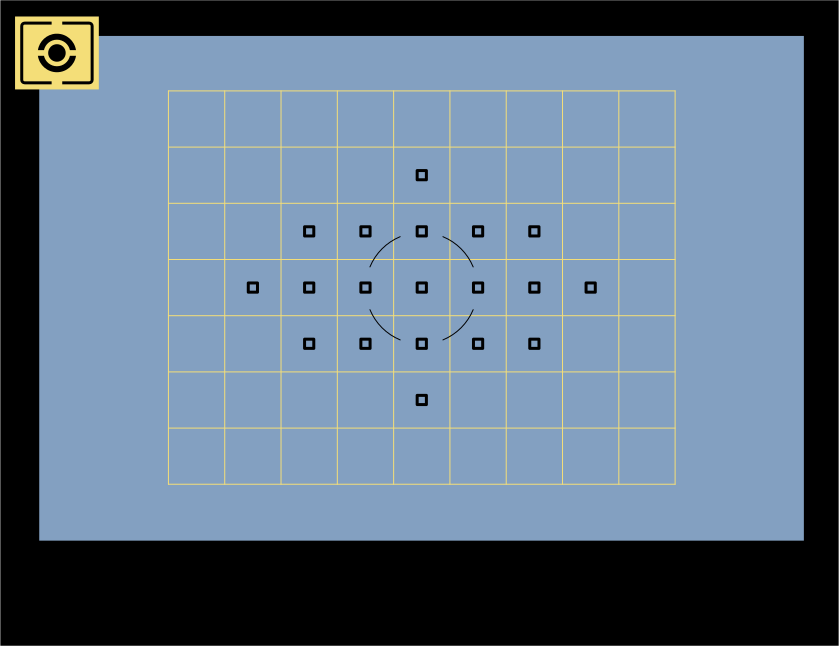
\includegraphics[width=0.65\linewidth]{figure/metering_evaluative.pdf}
% \caption{Mesure évaluative de l'exposition à partir des 63 zones représentées par un rectangle jaune. Les zones où la mise au point est faite auront un poids plus important dans l'évaluation globale.}\label{fig:metering-evaluative}
% \end{figure}

\subsubsection{Partielle}
La mesure est faite sur une zone au centre représentant environ 9\% de l'image (\reffig{fig:metering-partial}).

% \begin{figure}[htb]
% \centering
% \includegraphics[width=0.65\linewidth]{figure/metering_partial.pdf}
% \caption{L'évaluation partielle utilise un spot central qui représente environ 9\% de l'image.}\label{fig:metering-partial}
% \end{figure}

\subsubsection{Spot}
La mesure est faite sur un point central qui représente environ 3\% de l'image (\reffig{fig:metering-spot}).

% \begin{figure}[htb]
% \centering
% 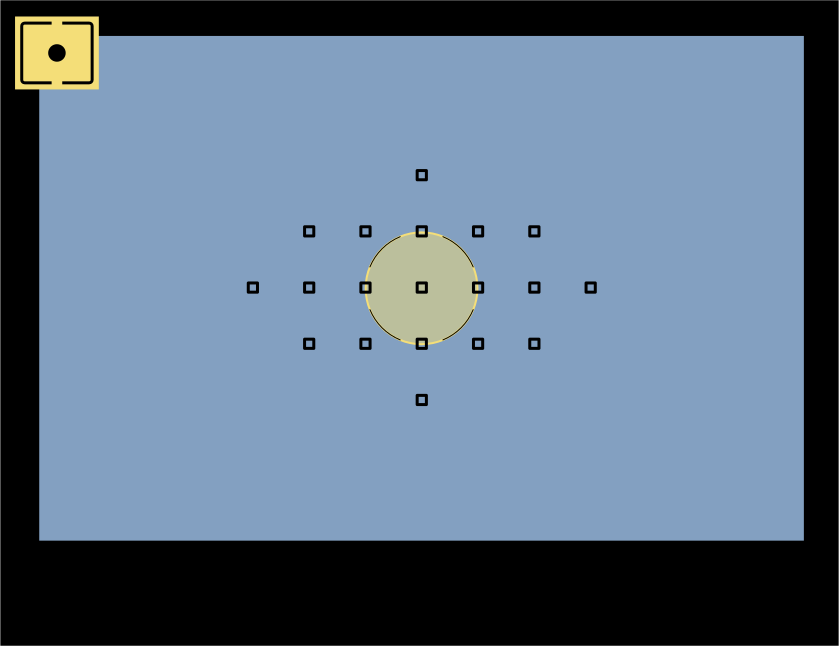
\includegraphics[width=0.65\linewidth]{figure/metering_spot.pdf}
% \caption{L'évaluation par spot base l'exposition sur une zone centrale représentant environ 3\%}\label{fig:metering-spot}
% \end{figure}

\begin{remarque}
Si la zone d'intérêt est au centre de l'image c'est parfait, mais si ce n'est pas le cas, il faut fait l'évaluation sur le point d'intérêt, puis bloquer l'évaluation avec le bouton \touche{AE lock}, et enfin recadrer l'image avant de prendre la photo.
\end{remarque}

\subsubsection{Priorité au centre}
Dans ce mode, l'évaluation du centre a plus d'importance que le reste de l'image (\reffig{fig:metering-central-weighted}). C'est typiquement intéressant pour faire des portraits. 

% \begin{figure}[htb]
% \centering
% 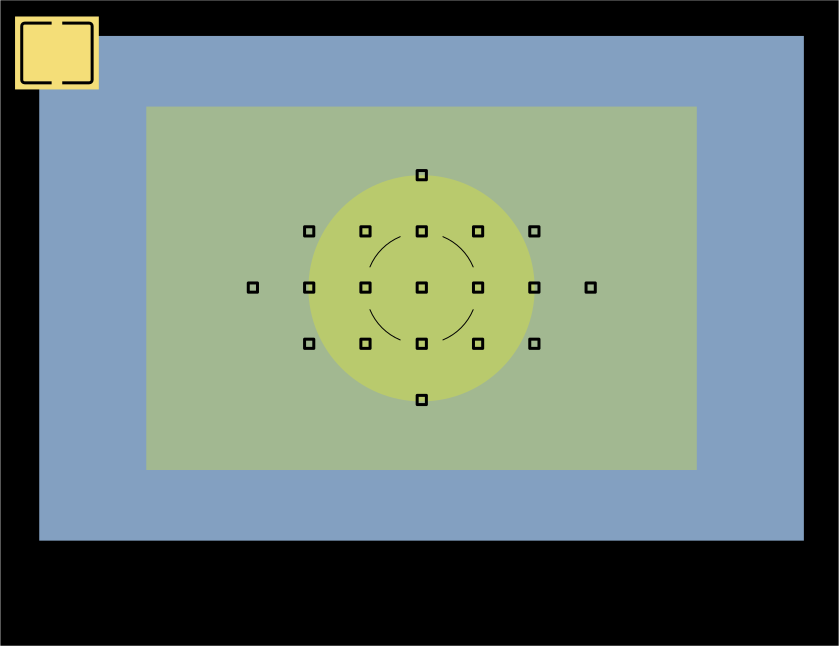
\includegraphics[width=0.65\linewidth]{figure/metering_central_weighted.pdf}
% \caption{Le mode d'évaluation \og central weighted\fg calcule l'exposition à partir de l'image complète, mais donne une importance plus grande à la zone centrale.}\label{fig:metering-central-weighted}
% \end{figure}

\subsection{Les différents modes d'un appareil photo}
\subsubsection{P}\index{mode!P}
C'est le mode automatique de l'appareil. Dans ce mode, l'appareil détermine tout seul la valeur d'ouverture et de vitesse d'obturation afin que la photo soit correctement exposée. Aucun contrôle sur ces valeurs. La roue crantée permet, une fois la mesure effectuée, de parcourir les combinaisons d'ouverture et de temps d'exposition qui permettent d'avoir la même exposition globale. 

\subsubsection{Tv}\index{mode!Tv}
Tv pour \textbf{Time Value}, c'est la priorité à la vitesse. Vous donnez une vitesse d'obturation, soit pour figer un sujet, soit pour un flou artistique (sur une fontaine par exemple) et l'appareil va déterminer l'ouverture qui permet d'avoir la bonne exposition.

Si l'ouverture clignote avec une valeur extrême, c'est qu'il est impossible d'exposer correctement la photo avec les valeurs choisies.

Dans ce mode, un Bracketing d'exposition (voir \refsec{sec:info-generales}) jouera sur l'ouverture pour avoir des expositions différentes, la vitesse d'obturation restant fixe.\index{bracketing}

\subsubsection{Av}\index{mode!Av}
Av pour \textbf{Aperture Value}, c'est la priorité à l'ouverture. Vous donnez une valeur d'ouverture, et l'appareil va déterminer la vitesse d'obturation nécessaire pour avoir la bonne exposition. 

Si la vitesse clignote avec une valeur extrême (30'' ou 1/8000), c'est qu'il est impossible d'exposer correctement la photo avec les valeurs choisies.

Dans ce mode, un Bracketing d'exposition (voir \refsec{sec:info-generales}) jouera sur l'ouverture pour avoir des expositions différentes, la vitesse d'obturation restant fixe.\index{bracketing}

\subsubsection{M}\index{mode!M}
Dans ce mode Manuel, vous donnez la valeur de la vitesse et de l'ouverture, au risque que l'exposition ne soit pas bonne. Lors de la mesure d'exposition, le 7D affiche la valeur EV (Exposure Value) à laquelle vous vous situez. Si vous êtes à 0, c'est que la photo est correctement exposée.

\subsubsection{B}\index{mode!B}
Bulb est un mode manuel, mais la différence essentielle, c'est que dans ce mode, le temps d'exposition correspond au temps de pression sur le bouton de prise de vue. Quand vous relâchez le bouton, la photo est prise.

\subsubsection{Modes personnalisés C1, C2, C3}
C'est l'une des choses les plus pratiques que j'ai trouvé pour l'instant. Ces 3 modes permettent de créer des réglages personnalisés. Concrêtement, vous réglez un mode de prise de vue ('P' par exemple), un style d'image, un mode d'évaluation de l'exposition, un mode rafale, la réduction des yeux rouges et ainsi de suite. Une fois que la configuration correspond à vos envies (pour des portraits par exemple), allez dans le 3\ieme menu des réglages, à ``Réglage utilisateur''. Sélectionnez ``enregistrer'' puis sélectionner le mode personnalisé (C1, C2 ou C3) dans lequel vous voulez enregistrer ces paramètres. 

Et voilà. Vous pouvez maintenant sélectionner ce mode via la molette de sélection des modes, sans avoir à rentrer tous les réglages à chaque fois. C'est un gain de temps énorme, et ça permet de ne rien oublier en plus, pour un mode spécifique.

Pour quelques exemples de modes, voir \refsec{sec:exemple_C1C2C3}.

\subsubsection{Infos générales sur ces modes}\label{sec:info-generales}
Si vous souhaitez utiliser le flash, il faut le sortir vous même, afin que l'exposition tienne compte de sa présence. 

La sensibilité ISO permettra de jouer sur l'exposition, à ouverture et vitesse constante. On peut aussi forcer l'ISO à une certaine valeur, pour empêcher l'appareil de modifier l'ISO quand il doit augmenter l'exposition (ne laissant comme degré de liberté que l'ouverture et la vitesse).

\bigskip

Il peut être utile d'utiliser l'AEB Bracketing (Auto-Exposure Bracketing) afin de prendre 3 photos avec des expositions différentes. C'est d'autant plus pratique qu'en mode rafale, rester appuyé sur le bouton va faire prendre les 3 photos à la suite (et arrêter la rafale automatiquement après). Cette technique est pratique pour tester différentes exposition, ou pour des photos en HDR (High Dynamic Range). 


\begin{figure}[htb]
\centering
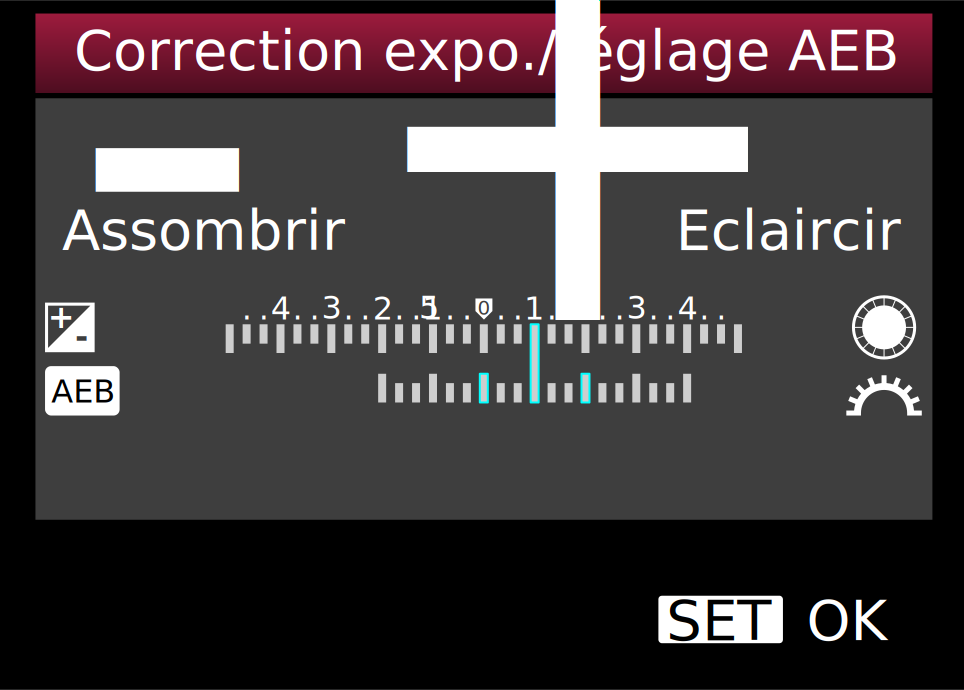
\includegraphics[width=0.65\linewidth]{figure/AEB_bracketing.pdf}
\caption{Mode qui permet le bracketing. La première échelle graduée permet de choisir la sous/sur exposition (maximum 5 stops pour le curseur central). La zone en dessous permet de choisir un bracketing autour de la valeur centrale (avec un écart maximal de 3 stops). Les traits encadrés de bleu sont les valeurs sélectionnées pour le bracketing.}
\end{figure}

\section{La mise au point}
Comme l'illustre \reffig{fig:mise_au_point}, en plus de la distance de mise au point, il y a ce qu'on appelle une profondeur de champ, qui est une zone autour de la distance de mise au point où les objets apparaîtront nets. 

\begin{remarque}
C'est à dire que le flou sur l'objet sera plus faible que la taille d'un pixel, il apparaîtra donc net, au même titre que les objets étant à la distance de mise au point.
\end{remarque}

\begin{figure}[htb]
\centering
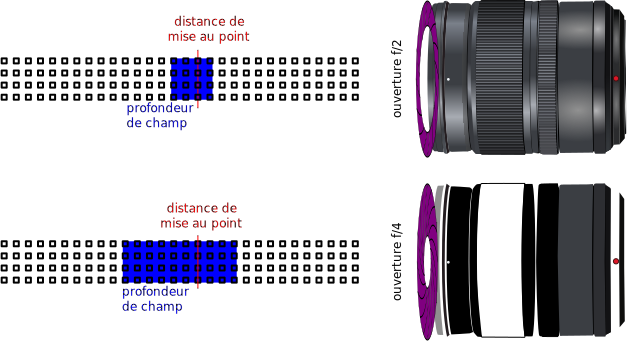
\includegraphics[width=0.65\linewidth]{figure/depth_of_field.pdf}
\caption{En fonction de l'ouverture, la profondeur de champ ne sera pas la même. Plus l'ouverture est grande, et plus la profondeur de champ est faible. À noter que la profondeur de champ n'est pas répartie symétriquement autour de la distance de mise au point. En gros, les deux tiers de la zone de netteté se situent derrière la distance de mise an point.}\label{fig:mise_au_point}
\end{figure}

\subsection{Modes autofocus}
En tout, le 7D possède 19 zones de mise au point. Mais il existe plusieurs modes qui se focalisent sur une ou plusieurs zones. Les figures \reffig{fig:autofocus_01} et \reffig{fig:AF_points_zone} représentent les différents modes d'autofocus accessibles. Les modes sont activables et désactivables via la fonction C.Fn III-06.

\begin{figure}[htb]
\centering
\hfill\subfloat[Dans ce mode, vous sélectionnez un point d'autofocus particulier, et la mise au point ne sera effectuée que sur ce point en particulier, les autres étant totalement ignorés.]{\label{fig:AF_points_single}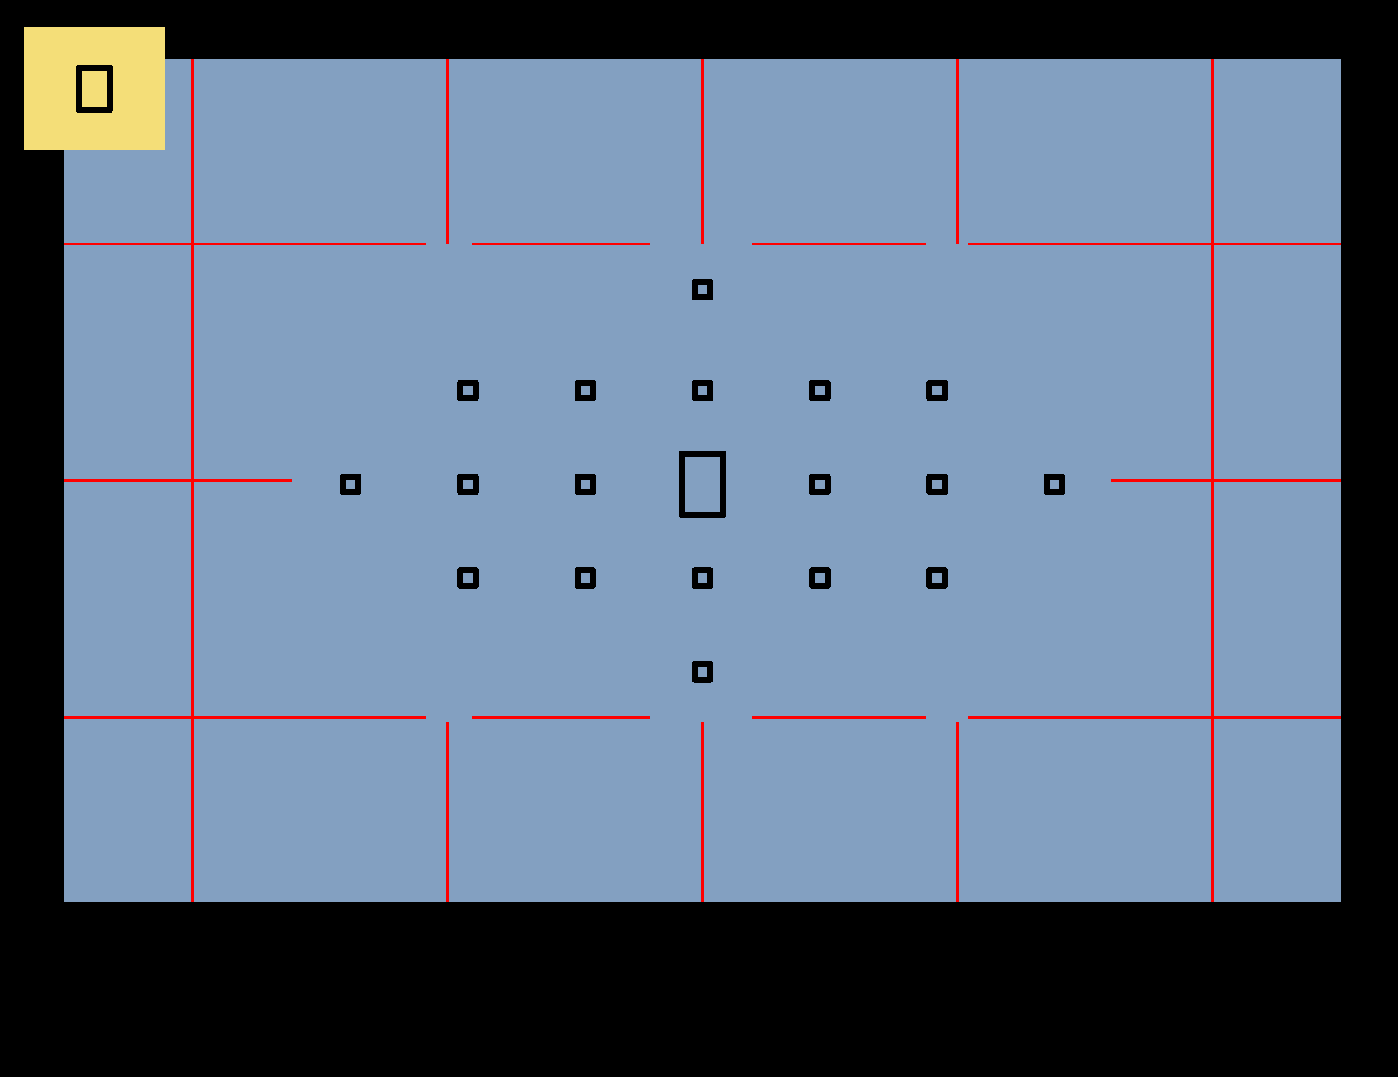
\includegraphics[width=0.35\linewidth]{figure/AF_points_single.pdf}}\hfill
\subfloat[Dans ce mode, vous sélectionnez un point d'autofocus particulier, et la mise au point ne sera effectuée que sur ce point en particulier, les autres étant totalement ignorés. La zone de mise au point est encore plus restreinte que quand vous sélectionnez un point d'autofocus normal.]{\label{fig:AF_points_spot}\includegraphics[width=0.35\linewidth]{figure/AF_points_spot.pdf}}\hfill~

\hfill\subfloat[Vous pouvez sélectioner un point d'autofocus, mais les points adjacents peuvent être utilisés pour un suivi de focus.]{\label{fig:AF_points_expansion}\includegraphics[width=0.35\linewidth]{figure/AF_points_expansion.pdf}}\hfill
\subfloat[Dans ce mode, la mise au point est effectuée automatiquement sur certains des 19 points d'autofocus du 7D. Ces points sont déterminés automatiquement.]{\label{fig:AF_points_automatic}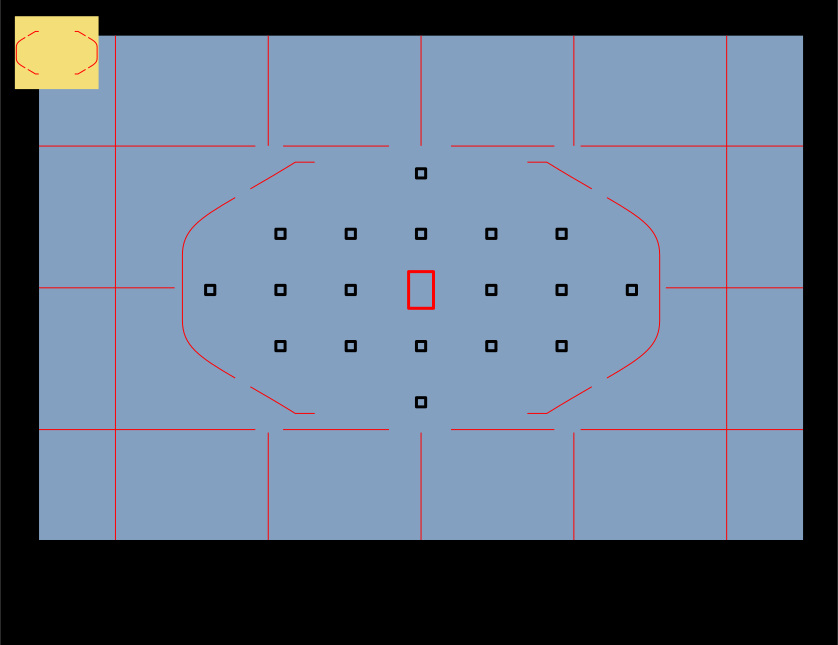
\includegraphics[width=0.35\linewidth]{figure/AF_points_automatic.pdf}}\hfill~
\caption{4 des 5 modes d'autofocus proposés par le 7D. Les modes sont activables et désactivables via la fonction C.Fn III-06.}\label{fig:autofocus_01}
\end{figure}

% \begin{figure}[htb]
% \centering
% 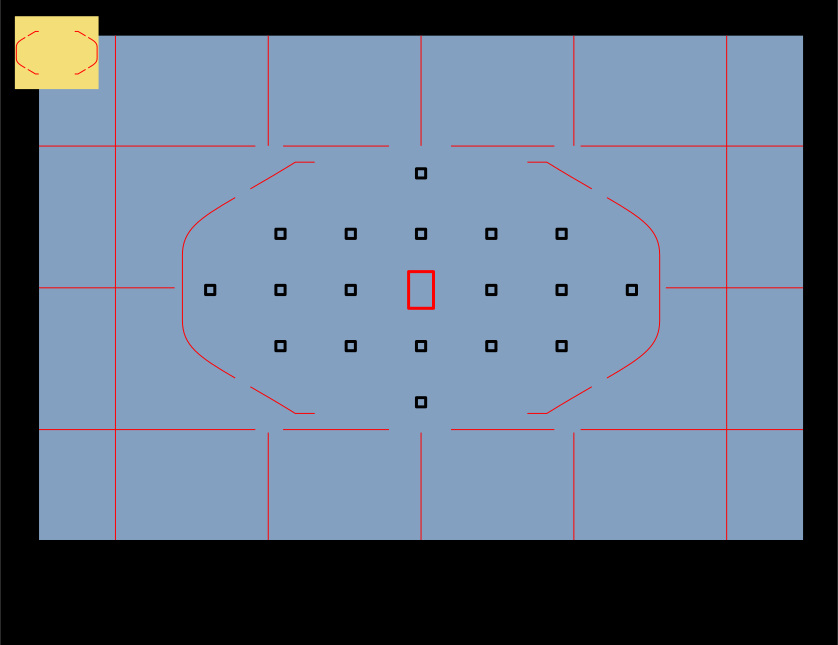
\includegraphics[width=0.35\linewidth]{figure/AF_points_automatic.pdf}
% \caption{Dans ce mode, la mise au point est effectuée automatiquement sur certains des 19 points d'autofocus du 7D. Ces points sont déterminés automatiquement.}\label{fig:AF_points_automatic}
% \end{figure}

% \begin{figure}[htb]
% \centering
% 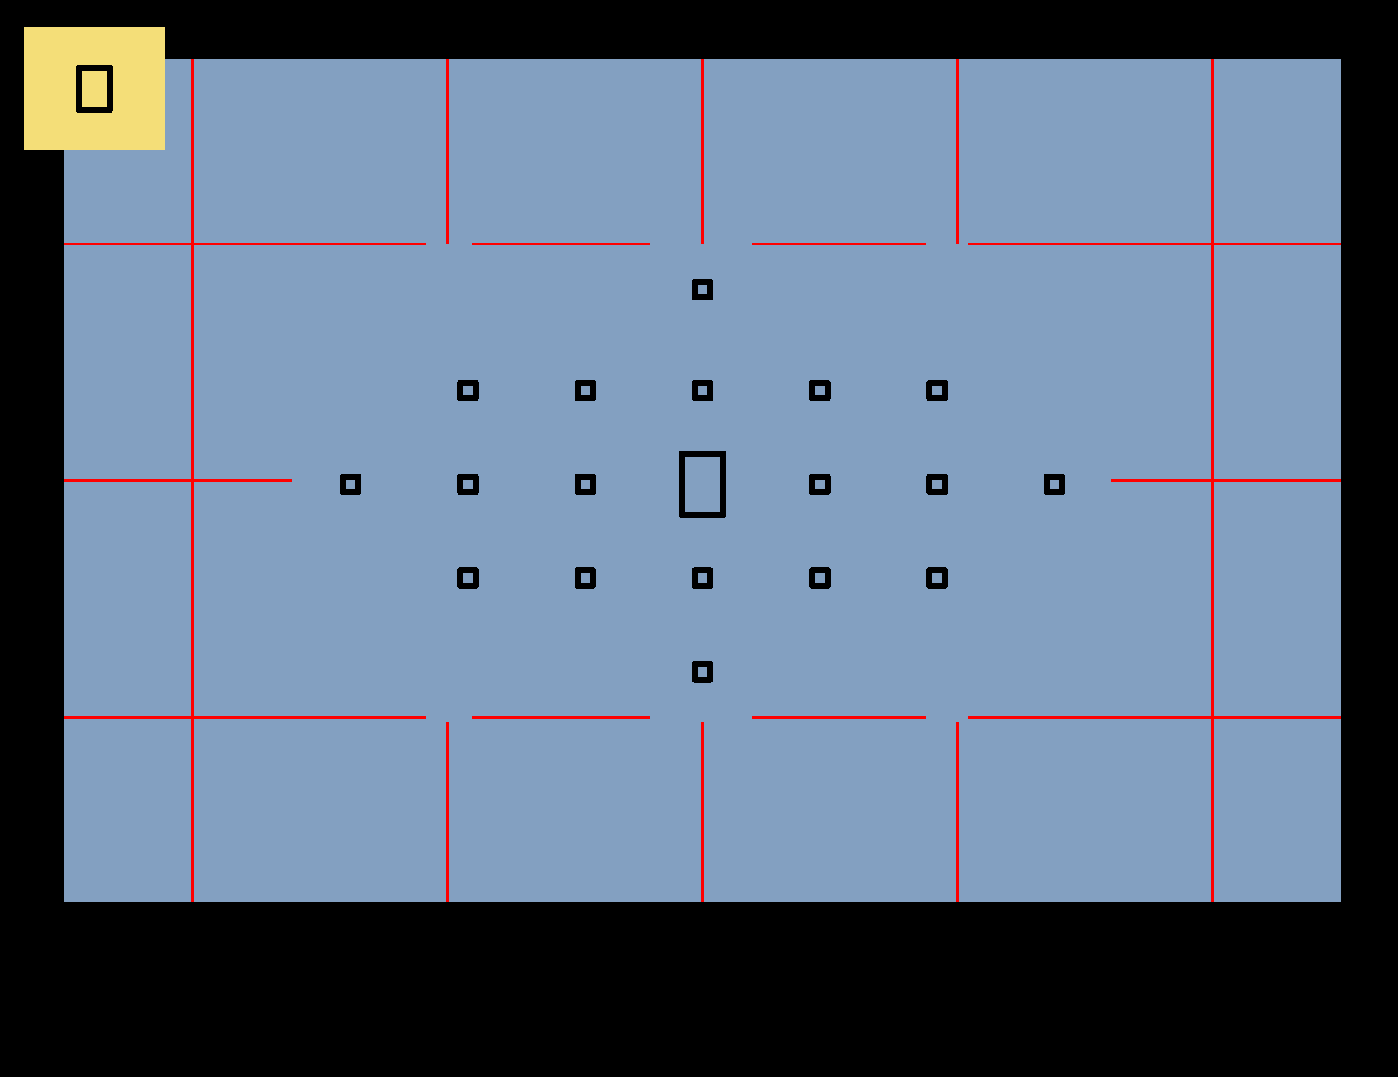
\includegraphics[width=0.35\linewidth]{figure/AF_points_single.pdf}
% \caption{Dans ce mode, vous sélectionnez un point d'autofocus particulier, et la mise au point ne sera effectuée que sur ce point en particulier, les autres étant totalement ignorés.}\label{fig:AF_points_single}
% \end{figure}
% 
% \begin{figure}[htb]
% \centering
% \includegraphics[width=0.35\linewidth]{figure/AF_points_spot.pdf}
% \caption{Dans ce mode, vous sélectionnez un point d'autofocus particulier, et la mise au point ne sera effectuée que sur ce point en particulier, les autres étant totalement ignorés. La zone de mise au point est encore plus restreinte que quand vous sélectionnez un point d'autofocus normal.}\label{fig:AF_points_spot}
% \end{figure}
% 
% \begin{figure}[htb]
% \centering
% \includegraphics[width=0.35\linewidth]{figure/AF_points_expansion.pdf}
% \caption{Vous pouvez sélectioner un point d'autofocus, mais les points adjacents peuvent être utilisés pour un suivi de focus.}\label{fig:AF_points_expansion}
% \end{figure}

\begin{figure}[htb]
\centering
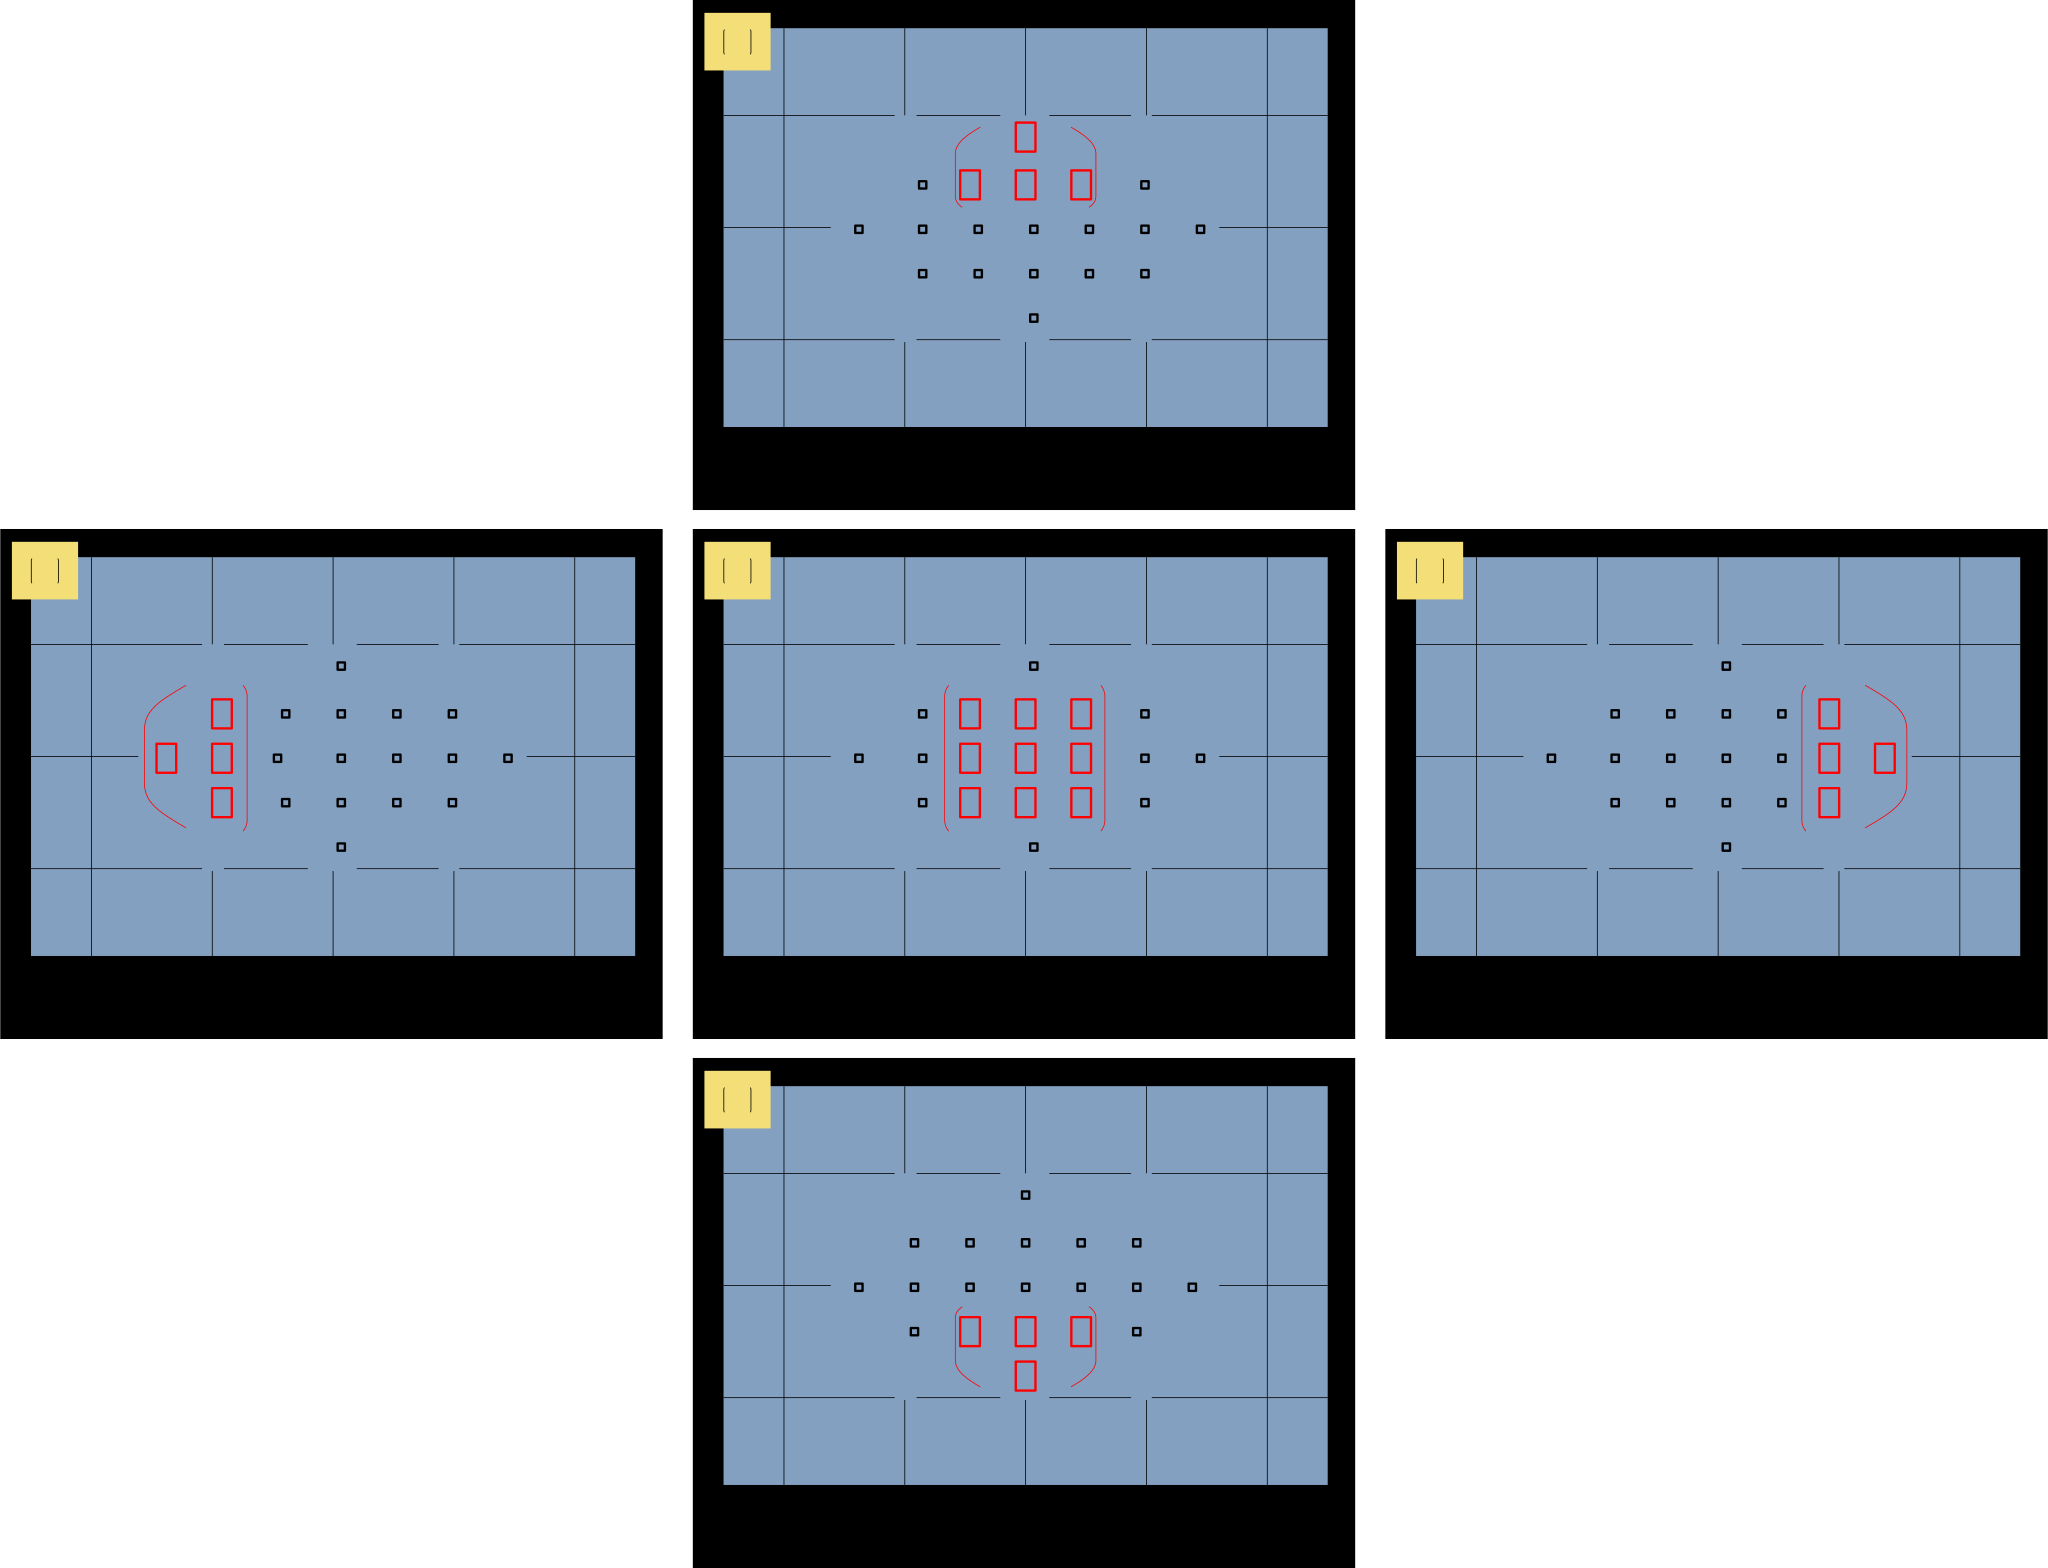
\includegraphics[width=\linewidth]{figure/AF_points_zone.pdf}
\caption{La mise au point est effectuée parmis les points d'autofocus d'une zone. 5 zones différentes sont à votre disposition. Les modes sont activables et désactivables via la fonction C.Fn III-06.}\label{fig:AF_points_zone}
\end{figure}

\subsection{Suivi autofocus}
\subsubsection{One shot}
Dans ce mode, la mise au point est effectuée une seule fois, lorsque vous pressez le bouton de prise de la photo à mi-course. Tant que l'appareil estime que la mise au point n'est pas faite, vous ne pourrez pas prendre la photo. Ce mode aura par conséquent un délai légèrement supérieur aux autres modes d'autofocus. On dit que ce mode donne la \textbf{priorité au focus}.

\begin{remarque}
En activant l'option C.Fn III-08, vous pourrez même voir dans le viseur les zones qui sont utilisées pour la mise au point, à l'aide de carrés rouge (ou noir). 
\end{remarque}

\subsubsection{AI Servo}
Ce mode correspond à la mise en point en continu. Tant que le bouton de l'obturateur est à mi-course, la mise au point se fera continuellement, s'efforçant de suivre le sujet mis au point au tout début.

Dans ce mode, rien n'empêchera la prise de vue, même si le sujet est légèrement défocalisé. On dit que ce mode donne la \textbf{priorité à l'obturateur}.

\subsubsection{AI Focus}
C'est en fait une combinaison des modes précédents. Par défaut, ce mode fait exactement la même chose que le mode One Shot. Mais si le sujet bouge, le mode passera automatiquement en AI Servo pour suivre le sujet. 

\subsection{Mise au point manuelle avec Live View}
Pour des cas précis, comme la mise au point manuelle quand le sujet et l'appareil sont fixes, le mode Live View peut être très pratique. En effet, avec la touche de zoom (tout en haut à droite de l'arrière de l'appareil) on peut zoomer sur l'image en x5 puis x10, ce qui permet d'avoir une mise au point manuelle beaucoup plus précise. Il n'est même pas nécessaire de rester en Live View une fois la mise au point faite. Il suffit de ne plus toucher à la bague de mise au point de l'objectif.

\section{Style d'image}
Le principe du style d'image est de donner des valeurs correctives à certains paramètres. \\
Ces paramètres sont les suivants :
\begin{itemize}
\item[\textbf{Netteté}] Ce paramètre permet de jouer sur l'impression de netteté de l'image. On peut ajuster ce paramètre entre 0 (pas d'ajout de netteté) à 7 (ajout très important de netteté). Gardez cependant à l'esprit que mettre ce paramètre au maximum ne sert à rien. Un peu de flou est nécessaire pour un rendu agréable de l'image, notamment pour empêcher l'effet Moiré\footnote{Rapidement, l'effet Moiré consiste en une alternance de ligne sombres et lumineuses dues à la superposition de deux réseaux. Dans le cas présent, superposition d'un réseau physique, dans le sujet qu'on photographie (un grillage ou tout autre motif régulier) et le réseau des pixels sur le capteur). }. Un exemple de l'effet Moiré est montré \reffig{fig:effet_moire}. De plus, un halo peut apparaître sur les bords de l'image si vous forcez trop la netteté.
\item[\textbf{Contraste}] Le contraste, de -4 (peu de contraste) à +4 (beaucoup de contraste) permet de déterminer le nombre de tons intermédiaires entre le noir le plus profond et le blanc le plus intense. Peu de contraste implique une image plate, tandis qu'un haut contraste pourra intensifier le rendu de l'image, au prix d'une perte de détails dans les ombres et les hautes lumières.
\item[\textbf{Saturation}] Ajustable de -4 (peu de saturationà à +4 (beaucoup de saturation), ce paramètre contrôle la richesse d'une couleur. Augmentez la saturation et la couleur s'accentuera, pour un ton rouge, il tendra plus vers le rouge vif et intense. Diminuez la saturation et le rouge sera plus fade, il tendra vers le rose puis vers le gris (sans saturation du tout, toutes les couleurs sont des niveaux de gris). Trop forcer la saturation entraine le phénomène de clipping (coupure) et certains détails pourront être perdus pour certaines couleurs (ceci est détectable avec les histogrammes RGB).
\item[\textbf{Teinte couleur}] Ce paramètre agit principalement sur les ton charnels, les rendant soit plus rouges (de 0 à -4) soit plus jaunes (de 0 à +4).
\end{itemize}

\begin{figure}[htb]
\centering
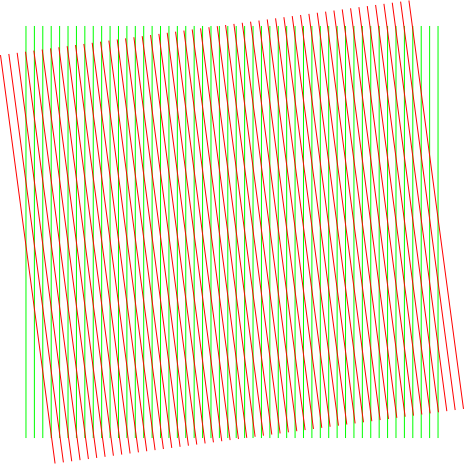
\includegraphics[width=0.25\linewidth]{figure/effet_moire.pdf}
\caption{Illustration de l'effet Moiré dans le cas d'une rotation entre deux réseaux (mais l'effet Moiré est quelque chose de plus général, même si le principe reste le même. On peut alors constater l'apparition d'une variation périodique verticale où le minimum correspond à l'intersection des lignes des deux réseaux.}\label{fig:effet_moire}
\end{figure}

\subsection{Standard}
C'est le style par défaut. Il applique des paramètres très génériques, comme la netteté accrue qui sont utilisables pour la plupart des photos. La valeur de la netteté est optimisée pour accroître la qualité de la photo, en limitant les cas de dégradation.

\subsection{Portrait}
La saturation est boostée pour des couleurs plus riches lors des portraits. Les tons sont plus chaleureux. Dans le même temps, la netteté est diminuée, pour donner une impression plus douce à la peau. 

\begin{remarque}
La netteté peut être augmentée pour donner une impression plus dure à la peau (notamment pour des portraits masculins) ou pour les sujets âgés des deux sexes, afin de marquer plus intensément les lignes du visage.
\end{remarque}

\subsection{Paysage}
Ce style augmente la saturation des bleus et verts et augmente aussi la netteté afin de rendre un paysage plus marqué et vif.


\subsection{Neutre}
C'est le même style que standard, mais avec la saturation et le contraste minimal. À utiliser par exemple quand les images sembles trop lumineuses ou contrastées (à la plage ou par grand soleil).

\subsection{Fidèle}
Ce style permet d'appliquer le moins de correction possible, afin d'être aussi fidèle que possible à ce que voient nos yeux (à condition que tout le reste soit réglé correctement bien sûr).

\subsection{Monochrome}
Style à utiliser pour faire des photos à un seul ton (noir et blanc par exemple). Différents réglages sont possibles, pour accentuer une teinte. À noter que les informations sur les couleurs seront toujours là si vous faites les photos en raw.

L'usage d'un filtre, va changer le contraste de la photo. En pratique, l'appareil va laisser passer uniquement les tons oranges, puis convertir ces tons en noir et blancs. En fonction du filtre, le ciel aura plus ou moins d'intensité, la peau, les feuilles des arbres, et ainsi de suite. ça permet d'agir de manière globale sur le rendu de la photo monochrome. 

À l'inverse, les tons vont donner une teinte au monochrome, en lieu et place de niveaux de gris classiques.


\section{Astuces diverses}
\subsection{Balance des blancs manuelle}
Dans un environnement spécial, comme un intérieur, avant un shooting complet, il est souhaitable de faire une photo d'un mur ou d'une zone blanche (avec focus manuel \textbf{MF}). 

Une fois la photo prise, il suffit d'aller dans le 2\ieme menu \og prise de vue\fg pour sélectionner \og balance des blancs personnalisée\fg. Il suffit ensuite d'appuyer sur \touche{SET}. 

Enfin, pour les photos où vous souhaitez utiliser ce réglage, il faut utiliser le mode personnalisé de balance des blancs (le symbole avec un carré plein et deux triangles non remplis en bas, à gauche et à droite).

\subsection{Quelques avantages du format raw}
Le format raw, en quelques mots, c'est un format qui contient les données brutes du capteur. Le traitement de l'appareil photo est effectué, mais la plupart des informations liées à ce traitement sont stockées avec le fichier, de sorte qu'ils puissent être modifiés après que la photo ait été prise. 

\bigskip

Le premier avantage évident est la profondeur de l'image. Dans une image JPEG, les couleurs d'un pixel sont stockées dans 24 bits (8 bits pour chaque couleur), autorisant un total de $16.7\times 10^{6}$ de couleurs différents (256 tons différents pour chacune des trois couleurs primaires). 

En raw, chaque couleur primaire est codée sur 14 bits, autorisant $4.4\times 10^{12}$ couleurs différentes. Ainsi, même après que la photo ait été prise, le fichier raw sera beaucoup plus tolérant et souple aux modifications de luminosité (et de manière générale, aux post-traitements). 

Par exemple, la valeur des paramètres suivants est modifiable a posteriori avec un fichier raw : 
\begin{itemize}
\item la balance des blancs (rendant faculatif l'utilisation d'un braketing de balance des blancs)
\item le style d'image (paysage, portrait etc...), le contrastes et toutes les caractéristiques définissant un style d'image sont corrigeable dans un fichier raw
\end{itemize}

\begin{attention}
Même avec un fichier raw, des pixels blancs ou noirs (un ciel cramé, ou des ombres sous exposées) ne seront pas rattrapables. Ces pixels là sont facilement identifiables avec les options appropriées dans l'appareil ou le logiciel, mettant en valeur les zones sur ou sous-exposées (un blanc ou un noir parfait resteront blanc ou noir quelle que soit la valeur de la correction de luminosité).
\end{attention}

\subsection{Les options à ne pas manquer du 7D}
Dans le 2\ieme menu bleu (de lecture). Il y a une option qui affiche les surexpositions quand on visualise les images. C'est rapidement indispensable. 

Toujours dans ce même menu, ``l'affichage collimateur AF'' est lui aussi indispensable. Il affiche lors de la visualisation (et de la prise de vue) les collimateurs AF où l'image est nette (où la mise au point est faite). 

\subsubsection{C.Fn I-06 Décalage de sécurité}
Si en mode Av ou Tv, les conditions de lumières changent et il n'est pas possible de prendre la photo avec la valeur que vous tentez d'imposer, l'appareil va modifier automatiquement cette dernière, ou en sélectionnant la valeur extrême pour l'autre paramètre libre. 

En gros, si vous avez une ouverture maximale de f/2.8, et si en mode Tv vous voulez une photo à 1/125s qui nécessiterait une ouverture de f/2 pour une bonne exposition, l'appareil changera pour 1/60s à la place, même si vous avez demandé 1/125s, et il prendre la photo à f/2.8.

\subsubsection{C.Fn I-07: Vitesse de synchronisation du flash en mode Av}\label{sec:vitesse_synchronisation}
La vitesse de synchronisation peut être un problème quand on utilise un flash, car l'exposition est calculée pour le flash, et n'a rien à voir avec l'exposition classique nécessaire s'il n'y avait pas de flash. 

En conséquence, la vitesse de synchronisation sert principalement à : 
\begin{itemize}
\item Figer le mouvement afin de ne pas avoir deux expositions pour les sujets en mouvement (l'exposition du flash, et l'exposition de la lumière ambiante)
\item Exposer correctement l'arrière plan qui lui n'est pas illuminé par le flash. 
\end{itemize}

En conséquence, cette option permet trois modes de fonctionnement pour le flash :
\begin{itemize}
\item[0 : Auto] L'appareil va adapter automatiquement la vitesse de synchronisation afin que l'arrière plan soit illuminé en partie par la lumière ambiante, en compensation du flash.
\item[1 : 1/250-1/60 sec. auto.] Dans ce mode, l'appareil va déterminer automatiquement la vitesse entre 1/250 et 1/60s, ceci afin d'éviter le bougé de l'appareil pendant des temps supérieurs à 1/60s.
\item[2 : 1/250s] Dans ce mode, l'exposition est automatiquement de 1/250s, rendant probablement l'arrière plan noir, mais empêchant le flou de bougé.
\end{itemize}

\subsubsection{C.Fn II-01: Réduction de bruit pour longue exposition}
Si l'option est activée, pour des temps d'exposition supérieurs à une seconde, une deuxième exposition, de durée équivalente, sera prise afin d'évaluer le bruit sur le capteur, et combiner les deux images à postériori.

\subsubsection{C.Fn II-03: Améliorer les détails dans les hautes lumières}
Cette option est particulièrement utile pour les photos de neiges ou de plage. Elle donne la priorité aux détails dans les zones lumineuses, au détriment des ombres, qui seront plus facilement cramées (et donc noire).

\subsubsection{C.Fn III-01: AI Servo sensibilité de suivi}
Le mode AI Servo permet de suivre un sujet et de corriger la mise au point tandis que ce dernier se déplace. Mais durant le suivi, un objet peut se retrouver devant le sujet que l'on souhaite suivre, et on peut ainsi perdre la mise au point. 

Cette option permet de modifier le délai pour une refocalisation (et donc un changement de sujet s'il reste trop longtemps dans le champ). Tout est une question d'équilibre, il n'y a pas de valeur miracle, et ça dépend vraiment du sujet à photographier. Mais voici quelques pistes : 
\begin{itemize}
\item \textbf{Slow} : Avec cette valeur, l'appareil va ignorer l'élément perturbateur pendant un long moment, avant de finalement refocaliser sur ce dernier. C'est utile quand les interruptions vont être fréquentes et longues. 
\item \textbf{Normal} Le temps est ici un peu plus court qu'avec la valeur ``lente'', c'est la valeur par défaut et généralement le meilleur choix pour des photos de sport, en effet, le délai peut perturber la vitesse d'autofocus le cas échéant.
\item \textbf{Fast} : En autorisant la refocalisation rapide, on peut accéder à des vitesses de mode rafale très importantes. 
\end{itemize}


\subsubsection{C.Fn III-03: AI Servo changement de focus}
Cette fonction permet de choisir le temps de latente avant que le sujet qui passe devant le sujet principal devienne le nouveau sujet d'intérêt.

Vous pouvez soit :
\begin{itemize}
\item Donner la priorité à la zone centrale, et tout objet passant devant agripera le focus, au risque de vous faire perdre la mise au point sur le sujet d'intérêt si un obstacle est passé devant. En photo sportive, le sujet d'intérêt sera souvent le sujet le plus proche, cette option est donc appropriée dans ces cas là.
\item Donner la priorité au premier sujet mis au point. Ainsi, même si quelque chose passe devant le sujet d'intérêt, le focus restera sur l'ancien objet, même plus lointain. Ainsi, des feuilles, branches, poteaux téléphoniques ne perturberont pas le focus. Ça peut être utile pour prendre en photo des animaux un peu cachés dans des fourrés.
\end{itemize}

\subsection{Exemples de modes personnalisés C1, C2, C3}\label{sec:exemple_C1C2C3}.
Ci-dessous, quelques configurations pour des types de photos, que vous pouvez alors mettre en mode personnalisé. Ce sont des modes que je modifie au fur et à mesure, et que j'affine donc. Ce n'est pas quelque chose de général, mais ça peut être utile ne serait-ce que comme base.

\subsubsection{Portrait}

\begin{tabular}{|c|c|p{5cm}|}
Mode Av & Ouverture f/4 & \\
Style d'image & Portrait & \\
Autofocus & AI Focus  & \\
C.Fn I-07 & 1 - Auto & Permet de limiter le flou de bouger lors de l'utilisation du flash\\
Focus & Choisir un seul point & \\
Exposition & priorité au centre & \\
Yeux rouges & Marche & \\
%TODO finir
\end{tabular}

\section{Techniques}
\subsection{Comprendre les effets des objectifs}
\subsubsection{Grands angles}
Les grands angles (courtes focales), vont avoir un grand champ de vision couvert. Tout va se passer comme si vous étiez plus loin que vous ne l'êtes réellement. En conséquence, vous mettre debout ou accroupi va complètement changer l'impression de la photo. De même si vous prenez en contre plongée (des gratte ciels par exemple).

\subsubsection{Téléobjectifs}
Les téléobjectifs, ou grandes focales, vont avoir tendance à écraser l'image, compressant les distances entre les différentes parties de l'image. Ça sera particulièrement à prendre en compte quand vous faites des portraits, le nez et les oreilles étant déformés par rapport à la forme normale du visage. 

De plus, un téléobjectif sera plus sensible aux vibrations. Généralement, une bonne approximation est d'avoir une vitesse d'obturation au moins inverse de la focale. C'est à dire que pour faire des photos avec un 100mm, il faut au moins avoir des vitesses de 1/100s (ou plus rapide).

Les objectifs sont sensibles aux lumières parasites arrivant par le coté de l'objectif sur la lentille frontale, provoquant des réflections (flares). Pour corriger ça, et améliorer le contraste, il faut utiliser le pare soleil, qui est spécialement conçu pour ça.

\subsubsection{Flou d'arrière plan : Bokeh}\index{bokeh}
Le Bokeh désigne le flou en dehors de la zone de netteté. Ce dernier n'aura pas forcément le même rendu en fonction de la qualité de l'objectif (et en particulier du diaphragme et son nombre de lamelle). Le Bokeh désigne les sortes de tâches qui vont se former pour chaque point qu'on aurait eu si la mise au point s'était fait à cet endroit de la composition. 

\subsection{Le Flash}
Le basique du flash est d'apporter plus de lumière que la lumière naturelle. Jusque là, j'enfonce des portes ouvertes. Mais il est important de comprendre certains principes avant de se lancer tête baissée dans le ``tout flash''. 

Si vous éclairez bêtement votre sujet de front, disons avec le flash interne à l'appareil, il y a de fortes chances pour que ce soit moche, pour plusieurs raisons : 
\begin{itemize}
\item toute la lumière formera un faisceau et éclairera principalement le sujet, laissant le reste tout noir.
\item La lumière sera dure
\item les yeux rouges s'il n'y a pas eu de pré flash qui permet de s'en prémunir
\item correction de balance des blancs à faire à postériori si vous n'avez pas pensé à modifier cette dernière avant la photo
\end{itemize}

S'il n'est pas vraiment important de comprendre comment est prise une photo dans un cas classique, ça le devient dans le cas du flash, car la durée d'exposition (la durée pendant laquelle il y a de la lumière flash) est beaucoup plus courte que le temps d'exposition. 

En effet, l'appareil photo possède deux régimes de mode d'exposition. L'appareil photo possède deux rideaux. 
\begin{itemize}
\item Pour des temps supérieurs à 1/250s (1/250s, 1/125s et ainsi de suite jusqu'à plusieurs secondes), l'appareil abaisse d'abord complètement le premier rideau (le capteur est alors soumis à la lumière), puis abaisse complètement le deuxième rideau. C'est ce qui est schématiquement représenté sur \reffig{fig:curtain_slow}.
\item Pour des temps inférieurs à 1/250s (1/500s, 1/1000s et jusqu'à 1/8000s dans le cas du 7D), l'appareil n'a pas le temps d'abaisser d'abord le premier rideau, puis faire l'exposition, puis abaisser le second rideau. Au lieu de ça, les deux rideau sont abaissé quasiment en même temps, avec un bref décalage qui permet l'exposition du capteur au fur et à mesure de la descente.
\end{itemize}

\begin{figure}[htb]
\centering
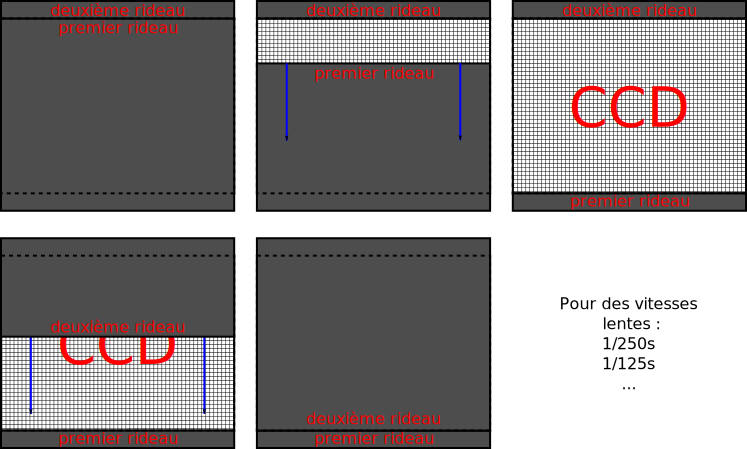
\includegraphics[width=0.45\linewidth]{figure/first_second_curtain_slow.pdf}
\caption{Illustration du déplacement des rideaux devant le capteur. Ce mode ne fonctionne que pour des temps d'exposition assez longs, supérieurs strictement à 1/250s. Pour ces temps d'exposition, l'appareil a le temps d'abaisser les rideaux l'un après l'autre. L'exposition se fait donc uniformément sur le capteur}\label{fig:curtain_slow}
\end{figure}

\begin{figure}[htb]
\centering
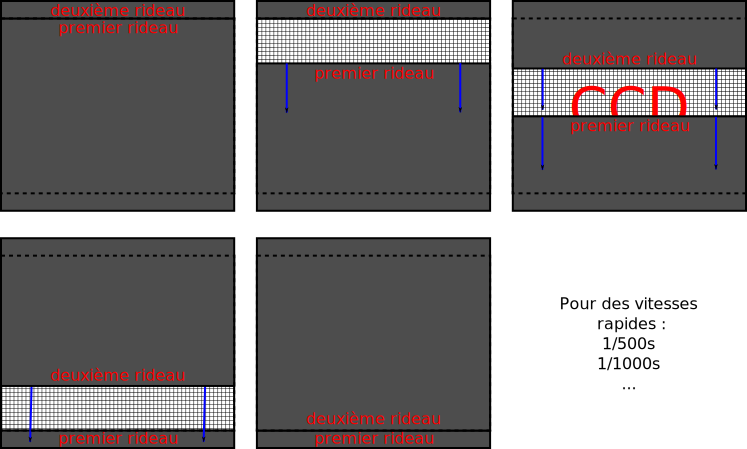
\includegraphics[width=0.45\linewidth]{figure/first_second_curtain_fast.pdf}
\caption{Illustration du déplacement des rideaux devant le capteur. Ce mode ne fonctionne que pour des temps d'exposition courts, inférieurs ou égaux à 1/250s. À ces vitesse là, l'appareil n'aurait pas le temps d'abaisser un rideau puis l'autre. Les deux rideaux sont abaissés en même temps, avec un décalage constant qui maintient une petite fenêtre d'ouverture, l'exposition se fait donc par balayage du capteur}\label{fig:curtain_slow}
\end{figure}

Ce petit détail a une importance cruciale dans le cas du flash. Il ne faut en aucun cas avoir une durée d'exposition inférieure à 1/250s (comme 1/500s par exemple), car le flash n'aurait pas accès à toute la surface du capteur, et certaines zones seraient non exposées. \refsec{sec:vitesse_synchronisation} détaille l'option qui permet de régler la vitesse de synchronisation du flash (pour le cas où on veuille exposer l'arrière plan à la lumière naturelle, ou simplement exposer le sujet sans se préoccuper du reste.

\subsubsection{Synchronisation du flash sur le 2e rideau}

Puisque l'exposition du flash est beaucoup plus courte que l'exposition totale de la photographie, il va y avoir deux images superposées, d'une part l'image figée par le flash, et d'autre part l'image provenant de la lumière ambiante, pendant le reste de l'exposition. Prenons le cas d'une voiture qui se déplace, le flash donnera une image nette de la voiture, tandis que la lumière ambiante laissera une trainée. Pour ce genre de cas, il est important de contrôler le moment, à l'intérieur même de l'exposition de la photo, où le flash sera déclenché. Ceci est contrôlable via le flash externe directement (il n'y a pas d'option sur le 7D apparemment) %TODO expliquer commment faire ça sur le 430EX

\subsubsection{Utilisation d'un flash déporté}
%TODO faire cette partie là (et noter les fonctions à activer sur le flash aussi)

\subsection{Réglages spécifiques à une scène}
Cette section a pour prétention de donner mes réglages pour certains types de photo. ÇA ne veut pas dire que c'est le must du must, mais c'est ce dont je me sers. Par exemple pour les feux d'artifices, j'ai loupé les 3/4 des photos à essayer des réglages avant de faire des photos potables avec les réglages que je donne, libre à vous d'essayer, ou de prendre mes réglages pour base. 

\subsubsection{Feux d'artifices}
Les contraintes sont multiples. La première chose, c'est qu'il y a peu de lumière, et que vous ne pouvez pas régler l'exposition sur le feu d'artifice, vu que c'est assez changeant. En conséquence, je prends le mode manuel. Je fixe une ouverture à f/5.6 et un temps d'exposition d'une seconde. Pourquoi une seconde? Parce que si vous faites des temps trop longs, vous pourrez avoir des photos surexposées et des fusées qui se superposent en une sorte d'amas difforme. La deuxième chose, c'est qu'avec des temps trop longs, si vous lancez la photo dans un moment creux, vous risquez de louper LA photo du finish en étant en train de finir une photo qui durait 15 secondes (ça m'est arrivé). 

Ce que je conseille : 
\begin{itemize}
\item Utilisation d'un trépied
\item Effectuez la mise au point automatique au début, puis bloquez en mode manuel. La mise au point doit être quasiment à l'infini si vous êtes suffisamment loin du feu d'artifice. Ceci vous évitera les problèmes de mise au point au cours de prise de vue, si l'appareil veut faire la mise au point un peu avant l'explosion, alors que tout est noir.
\item Mode manuel
\item ouverture f/5.6
\item exposition 1/2 seconde
\item mode rafale (pour prendre des photos en continu)
\item sensibilité ISO 100
\item balance des blancs neutre
\end{itemize}

\begin{remarque}
Pensez à ne pas prendre de photo pendant les temps mort, histoire d'économiser la carte mémoire. J'ai perdu le finish avec un \og Carte Pleine\fg\dots
\end{remarque}


\printindex
\end{document}